
%(BEGIN_QUESTION)
% Copyright 2007, Tony R. Kuphaldt, released under the Creative Commons Attribution License (v 1.0)
% This means you may do almost anything with this work of mine, so long as you give me proper credit

Shown here is the response of a process to a series of step-changes on the controller output (all made with the controller in ``manual'' mode).  Based on your observations, what can you ascertain about the process and its related instrumentation?

$$\includegraphics[width=15.5cm]{i01651x01.eps}$$

Is this process response a potential problem?  If so, what type of problem is it?

\underbar{file i01651}
%(END_QUESTION)





%(BEGIN_ANSWER)

The process (as a whole) has a variable gain.  If the process has a variable gain, it means the entire loop gain will increase and decrease depending on the PV's value.  This means the loop will be less stable at some PV values than at others.

This may be due to a severe nonlinearity in the transmitter or in a signal transducer, a control valve with a nonlinear installed characteristic (in this case, an equal-percent {\it installed} characteristic -- very unlikely), or something inherent to the process itself (most likely). 

To counter this gain instability, the controller (or some other element in the control loop) must be configured to have an inverse gain response, so that the loop gain always remains constant.  An {\it adaptive gain} controller may be used for this purpose, or perhaps a different valve characteristic may be installed.

%(END_ANSWER)





%(BEGIN_NOTES)


%INDEX% Control, PID tuning: step change (output) revealing variable gain

%(END_NOTES)


